% !TEX encoding = UTF-8 Unicode

\documentclass[a4paper]{article}

\usepackage{color}
\usepackage{url}
\usepackage[T2A]{fontenc} % enable Cyrillic fonts
\usepackage[utf8]{inputenc} % make weird characters work
\usepackage{graphicx}
\usepackage{subfig}

\usepackage[english,serbian]{babel}
%\usepackage[english,serbianc]{babel} %ukljuciti babel sa ovim opcijama, umesto gornjim, ukoliko se koristi cirilica

\usepackage[unicode]{hyperref}
\hypersetup{colorlinks,citecolor=green,filecolor=green,linkcolor=blue,urlcolor=blue}

%\newtheorem{primer}{Пример}[section] %ćirilični primer
\newtheorem{primer}{Primer}[section]

\begin{document}

\title{Bitcoin u 2022. godini\\ \small{Seminarski rad u okviru kursa\\Tehničko i naučno pisanje\\ Matematički fakultet}}

\author{Lazar\\ @alas.matf.bg.ac.rs\and Tanja Damnjanović\\mi19377@alas.matf.bg.ac.rs\and Aleksa Marković\\mi20244@alas.matf.bg.ac.rs\and Miljan Lješnjak\\mi22359@alas.matf.bg.ac.rs }
\date{21.~novembar 2022.}
\maketitle


\tableofcontents


\newpage

\section{Uvod}
\label{sec:uvod}
Poslednjih decenija nagli razvoj tehnologije i interneta omogućio je početak elektronske trgovine. U početku se trgovina na internetu oslanjala na finansijske institucije koje su bile posrednici tokom obrade plaćanja. Iako  je takav sistem uglavnom bio dobar, još uvek su postojale mane u pogledu poverenja. Bio je potreban sistem bez posrednika koji dopušta direktnu trgovinu između korisnika. Taj koncept se pojavljuje 2008. godine sa prvim i glavnim predstavnikom pod nazivom  Bitkoin \textbf{(eng. Bitcoin)} po kome su kasnije zasnovane ostale digitalne, odnosno virtualne valute. Neki entuzijasti bitkoina jednostavno vide kriptovalute kao zabavnu imovinu za trgovanje, dok drugi veruju da bi mogla postati univerzalna valuta digitalnog sveta.
\\

\section{Istorija i nastanak}
\subsection{Početak}
Kriptovaluta je oblik digitalnog novca. Za stvaranje i beleženje njenih transakcija koriste se kriptografski mehanizmi koji omogućavaju različitim korisnicima koji nemaju poverenje jedni u druge da veruju sistemu. Bitkoin je prvi primer kriptovalute. Jedinice valute zvane bitkoin koriste  se za prenos vrednosti među korisnicima u bitkoin mreži. Predstavljen je 2008. godine sa člankom pod nazivom ``Bitcoin: A Peer-to-Peer Electronic Cash System'' čiji je autor poznat samo pod pseudonimom  ``Satoshi Nakamoto''. Sistem peer-to-peer znači da korisnici mogu trgovati direktno, bez posrednika. Namera je bila ostvariti kontrolu nad finansijama stvaranjem stabilne, sigurne, svetski prihvatljive valute. 
Početkom 2009. godine i prvi bitkoini se puštaju u promet. Primalac prve bitkoin transakcije je bio Hal Finej. Finej je preuzeo bitkoin softver na datum izlaska softvera, i 12. januara 2009. godine je primio 10 bitkoina od Nakamota. Prva poznata komercijalna transakcija se dogodila 22. maja 2010. godine kada je Lazlo Hanjec kupio 2 pice iz Papa Džon picerije za 10,000 bitkoina. Danas bitkoin zajednica proslavlja taj datum kao dan pice. 
Identitet autora ostaje nepoznat a neke popularne pretpostavke su da je to tim stručnjaka  ili osoba koja se povukla da bi zaštitila svoju privatnost i pre povlačenja iz javnosti 2010. godine prepustila glavnu ulogu Gavinu Andresenu koji je sad vođa projekta. Tokom godina nekoliko osoba je tvrdilo da su pravi Satoshi Nakamoto ali nijedna nije mogla da obezbedi dovoljan dokaz da podrži tu tvrdnju.

\subsection{Uspon bitkoina}
Prvih godina, bikoin nije imao značajnu vrednost a aktivnosti su bile slabe i uglavnom su se svodile na razmenu bitkoina između ljudi koje je zanimala kriptografija. Prvi veći korisnici su bili na crnom tržištu. Sredinom 2011. godine dolazi do prvog značajnog skoka popularnosti, ujedno i vrednosti. U narednoj godini tokom kiparske finansijske krize bitkoin dostize čak 266\$, otvaraju se prve online menjačnine kriptovaluta i neke radnje počinju da prihvataju bitkoin kao validno sredstvo plaćanja. Nastaje Bitkoin Fondacija radi promovisanja razvića i shvatanja bitkoina. Razvitak se nastavlja 2013. godine kada ``Baidu'' počinje da prihvata bitkoin za svoje usluge bezbednosnih servisa. Ubrzo se otvara i prva bitkoin menjačnica ``BTC China'' koja nadjačava do tada najpopularniju menjačnicu ``Mt. Gox''. Ubrzo posle toga Senat Sjedinjenih Amreričkih država priznaje kriptovalute kao legitimno sredstvo plaćanja i u tom danu bitkoin skače na 1100\$. Uticaj Senata na cenu bitkoina najbolje prikazuje grafikon bitkoin cene, prikazan na slici \ref{fig:grafikon}.


\begin{figure}[h!]
	\begin{center}
		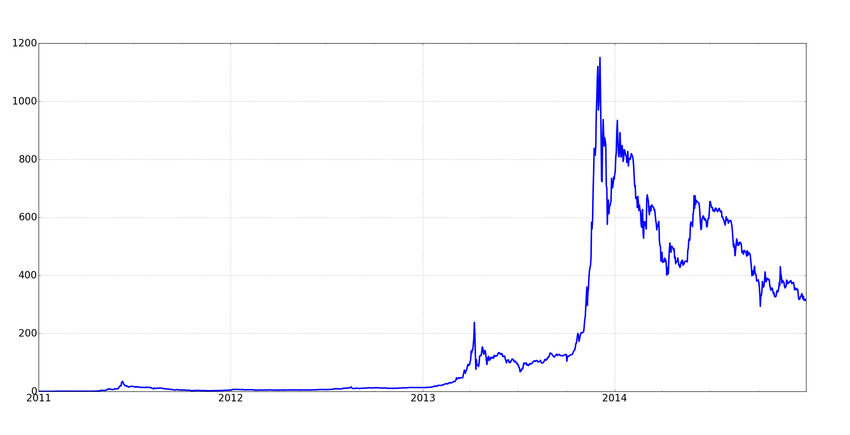
\includegraphics[scale=0.4]{chart.png}
	\end{center}
	\caption{Cena bitkoina od 2011. do 2015. godine}
	\label{fig:grafikon}
\end{figure}

\section{Princip rada Bitkoina}
\label{sec:princip_rada}

Bitkoin je izgradjen na distribuiranom digitalnom zapisu koji se zove Blokčejn \textbf{(eng. Blockchain)}. Kao što naziv implicira, blokčejn predstavlja povezano telo podataka, sastavljeno od jedinica koje se nazivaju blokovi. Blokovi sadrže informacije o svakoj transakciji, uključujući datum i vreme, ukupnu vrednost, kupca i prodavca i jedinstveni identifikacioni kod za svaku razmenu. Unosi su nanizani hronološkim redom, stvarajući digitalan lanac blokova.\cite{princip_rada} U tabeli \ref{tab:tabela_blok} su prikazane informacije koje se čuvaju u blokovima.
\\


\begin{table}[h!]

\begin{center}
\caption{Struktura blokova u blokčejnu.}

\captionsetup[subfloat]{labelformat=empty}
\subfloat[Block n]{
\begin{tabular}{|c|} \hline
Block Header \\ \hline
Transaction Counter\\ \hline
List of Transactions \\ \hline
\end{tabular}
}
\quad
\subfloat{
\begin{tabular}{ccc}
\\ 
$\longrightarrow$ \\
\\
\end{tabular}
}
\quad
\subfloat[Block n+1]{
\begin{tabular}{|c|} \hline
Block Header \\ \hline
Transaction Counter\\ \hline
List of Transactions \\ \hline
\end{tabular}
}

\label{tab:tabela_blok}
\end{center}
\end{table}

Jednom kada se blok doda u blokčejn, on postaje dostupan svima koji žele da ga vide, delujući kao javna knjiga transakcija kriptovaluta.
\\
Blokčejn je decentralizovan, što znači da ga ne kontroliše nijedna organizacija. Niko ga ne poseduje, ali svako može da ga koristi i da doprinese njegovom razvoju. Kako ga različiti ljudi ažuriraju, kopija koju pojedinac poseduje se takodje ažurira.

Iako ideja da svako može da uredjuje blokčejn može zvučati rizično, to je zapravo ono što bitkoin čini pouzdanim i sigurnim.
\\
\\
Da bi blok trasakcije bio dodat bitkoin blok lancu, mora da bude verifikovan od strane velikog broja vlasnika bitkoina, a za svakog korisnika koristi se jedinsveni verifikacioni kod.
\\
\\
Verifikacioni kodovi su dugi, nasumični brojevi, što njihovo lažiranje ili zloupotrebu predstavlja izuzetno teškim. Nivo statističke nasumičnosti blokčejn verificionih kodova, koji su potrebni za svaku transakciju, u velikoj meri smanjuje rizik da svako može da vrši razne zloupotrebe i lažne bitkoin transakcije.


\section{Socioekonomski uticaj bitkoina}

\subsection{Energija}

Rudarenje bitkoina zahteva mašine sa puno procesorske snage, pa je samim tim velika potrošnja energije neophodna da bi se hardver poput grafičke kartice pokretao, iako su novije komponente sve više i više energetski efikasne. Pored mašina, rudari i kompanije za rudarenje sa velikim sistemima često imaju potrebu za jakim uređajima za rashlađivanje koje potpomažu performanse. Energija koja se troši prilikom rudarenja bitkoina raste zajedno sa bitkoin mrežom.

Gledajući energiju koja se godišnje potroši na rudarenje bitkoina, možemo videti da ona prevazilazi količine koje godišnje potroše čitave države. Bitkoin je 2019. godine potrošio oko 87.1 TWh\footnote{Teravat-sat} električne energije, što je približno količini koju je te godine potrošila Belgija.  \cite{energijapotrosnja}


Ovolika potrošnja energije ima mnogo posledica. Mapa rudarenja bitkoina u periodu 2019-2020, na osnovu geolokacije rudara ukazuje da je skoro 70\% rudarenja rađeno u Kini. \cite{energijakina}

Kako se Kina najviše oslanja na energiju dobijenu iz fosilnih goriva, može se reći da bitkoin dovodi do emitovanja značajne količine gasova staklene bašte.

Ova otkrića imala su negativan efekat na reputaciju bitkoina, pošto sve više ljudi brine o klimatskim promenama i preferira zelenu energiju. Jedan od izazova za bitkoin biće potrošnja energije i prelaženje na čistije i održivije energije.


\subsection{Cene i zalihe hardverda }

Grafičke kartice jedna su od najčešćih hardverskih komponenti koje se koriste za rudarenje bitkoina. Većina rudara koristi više od jedne grafičke kartice za njihov sistem, a česta je i pojava čitavih farmi \ref{fig:farma} (industrijski objekti namenjeni rudarenju). To je neophodno da bi rudarenje uopšte bilo isplativo i iz istog razloga rudari teže da nabave najnovije kartice po njihovom izlasku.


\begin{figure}[h!]
	\begin{center}
		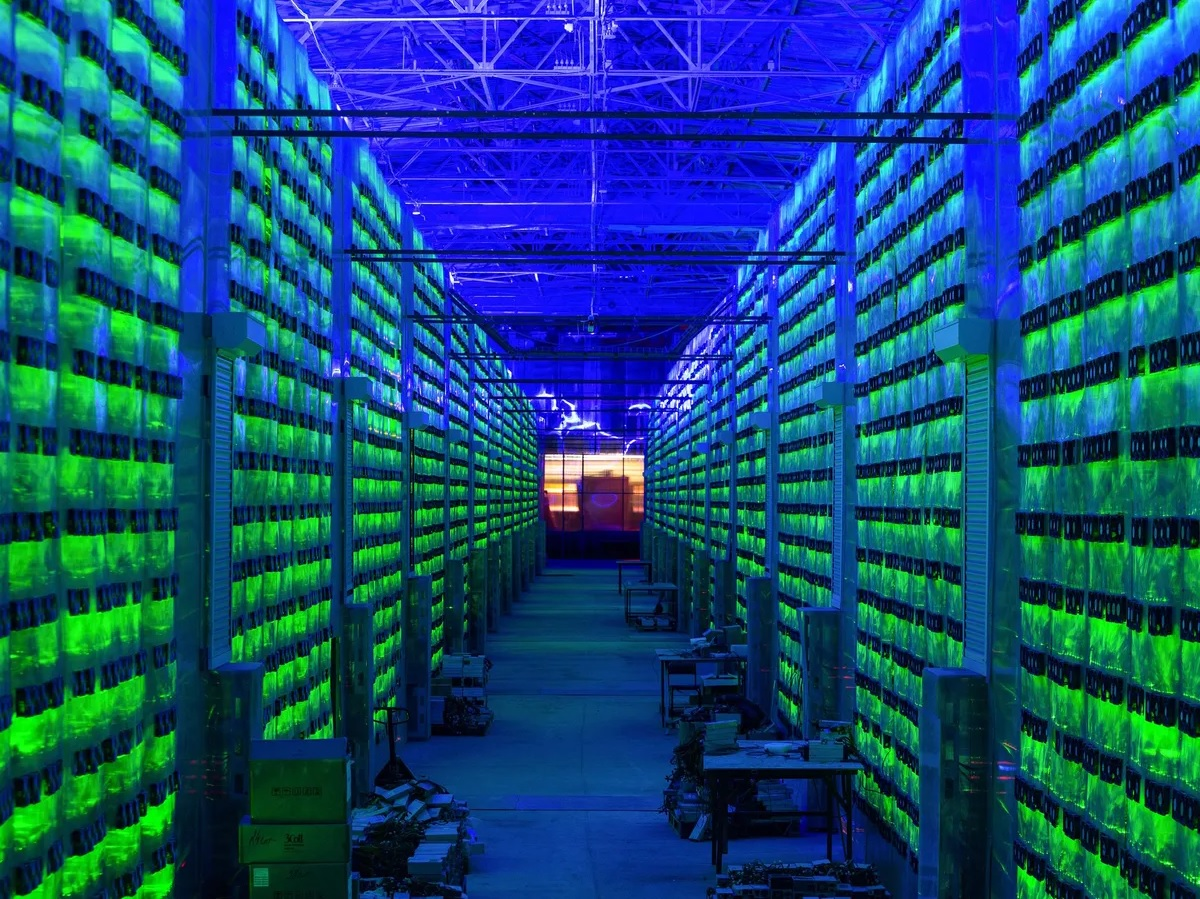
\includegraphics[scale=0.25]{farma.jpg}
	\end{center}
	\caption{Farma za rudarenje u Rusiji}
	\label{fig:farma}
\end{figure}

Ovo je jedan od razloga zbog kojih postoji nestašica grafičkih kartica, i to je problem koji se znatno pogoršava sa porastom popularnosti bitkoina i generalno kriptovaluta. Najnovije i najjače grafičke kartice većinski kupuju kompanije specijalizovane za rudarenje i individualni rudari. Maloprodaje iskorišćavaju činjenicu da proizvođači ne mogu da ispune ogromnu potražnju, te podižu cene do čak tri puta više od preporučene.

Bočni efekat ovog problema je veliki uticaj na polovno tržište grafičkih kartica. Kako nema grafičkih kartica u zalihama, rudari se okreću ovom tržištu i masovno kupuju polovne kartice, s obzirom da je često potrebno više starijih modela grafičkih kartica da bi bile isplative koliko i najnoviji modeli. Ovo iskorišćavaju i ljudi koji prodaju svoje korišćene kartice da podignu cene do te mere, da ih prodaju za više para nego što su ih platili nove.

Sve ovo skoro onemogućava prosečnom potrošaču da kupi grafičku karticu. U pokušaju da oslabe ove efekte, proizvođači uvode razne mere. NVIDIA, jedna od najvećih proizvođača grafičkih kartica, odlučila je da krene sa proizvodnjom grafičkih kartica specijalizovanih za rudarenje. Takođe je umanjila performanse rudarenja novih grafičkih kartica, koje su prvenstveno namenjene za video igrice, tako što im je umanjila hash rate. Ovo je dovelo do kritika od strane potrošača, na račun toga da NVIDIA svoju pažnju posvećuje grafičkim karticama namenjenim za rudarenje, dok stare linije ostavlja po strani. Takođe su ove odluke kritikovane da nove grafičke kartice neće imati preprodajnu vrednost i da će biti jednokratne.

\subsection{Monetarni sistem i politika}

Trenutno bitkoin skoro da nema uticaj na monetarne sisteme, s obzirom da je tržišna kapitalizacija bitkoina u svom vrhuncu bila oko 1.2 biliona američkih dolara, što je više od 5 puta manje od tržišne kapitalizacije bankarskog tržišta. Takođe, čak i centralne banke koje eksperimentišu sa kriptovalutama ne planiraju da koriste blokchain za njihove projekte, jer ga smatraju nestabilnim za infrastrukturu nacionalnih valuta. Kako se bitkoin oslanja na blokchain to ga čini nepogodnim, i samim tim neće imati uticaj na buduće planove monetarnog sistema.

Neke vlade se osećaju ugroženo od strane bitkoina iz razloga što bitkoin nema centralnu vlast i zato što može da destabilizuje autoritet centralnih banaka ili čak i samih vlada. Anonimnost koju pruža bitkoin može se koristiti za zaobilaženje raznih kontrola, pranje novca ili ilegalnu kupovinu. Zbog toga političari neretko ukazuju na probleme i mane bitkoina, poput potrošnje energije, sa ciljem da pokvari poverenje ljudi u njega. Sa druge strane, neki političari biraju da kritikuju način na koji se bitkoin oporezuje i razmenjuje sa ciljem da odvrate ljude od investiranja. To ne ide u prilog bitkoinu, koji još uvek većina investitora smatra za rizičnu investiciju.


\section{Zaključak}

U ovom radu smo videli tehničke i ekonomske osobine bitkoina, kao i njegov potencijal da se takmiči sa trenutnim monetarnim sisteom.
Zahvaljujući  bitkoinovoj decentralizovanoj arhitekturi, zasnovanoj na blokčejnu, bitkoin pruža visok nivo bezbednosti i transparentnosti, kojima ne mogu da pariraju tradicionalni finansijski sistemi. Zbog njih je bitkoin stekao određenu dozu poverenja i podrške od korisnika.

Ipak još uvek postoje problemi poput volatilnosti njegove cene i njegov pravni status, kao i upotreba bitkoina za ilegalne aktivnosti.
Međutim kako sve više ljudi i biznisa prihvata bitkoin, njegov potencijal kao alternativna valuta samo raste.

\clearpage

\addcontentsline{toc}{section}{Literatura}
\appendix

\iffalse
\bibliography{seminarski} 
\bibliographystyle{plain}
\fi

\begin{thebibliography}{9}

\bibitem{princip_rada} Nakamoto Satoshi. \emph{Bitcoin: A Peer-to-Peer Electronic Cash System}. bitcoin.org

\bibitem{energijapotrosnja} Alex de Vries. \emph{Bitcoin’s energy consumption is underestimated: A market dynamics approach}. Energy Res. Social Sci., vol. 70, Dec. 2020.

\bibitem{energijakina} Alex de Vries. \emph{IEA (2019), Bitcoin energy use - mined the gap}.  IEA, Paris, https://www.iea.org/commentaries/bitcoin-energy-use-mined-the-gap 



\end{thebibliography}



\end{document}
